\documentclass[10pt, aspectratio=1610, handout]{beamer}
\usepackage{common}

\title[VFI, PFI and DP]{
  \textbf{Value Function Iteration, Policy Function Iteration and Direct Projection}
}

\subtitle[Macro 3: TA\#2]{
  \textbf{Macroeconomics 3:} TA class \#2
}

\author[A.~Pasqualini]{
  Andrea Pasqualini
}

\institute[Bocconi]{Bocconi University}

\date{
  15 February 2021
}

\begin{document}

  \begin{frame}
    \maketitle
  \end{frame}

  \begin{frame}
    \frametitle{Plan for Today}

    Objective: \textbf{Solve numerically for $V(K)$ and $K'(K)$}

    \vfill\pause

    Operating example: Neoclassical Growth Model (deterministic version)
    \begin{align*}
      V(K) \equiv \max_{C, K'} &\; \frac{C^{1 - \gamma}}{1 - \gamma} + \beta V(K') \\
      \text{s.t.} &\;
      \begin{cases}
        C + K' \leq K^\alpha + (1 - \delta) K \\
        C, K' > 0
      \end{cases}
    \end{align*}

    \vfill\pause

    \begin{columns}[T]
      \begin{column}{0.45\textwidth}
        Objects of interest
        \begin{itemize}
          \item Policy functions (for simulations)
          \item Value function (for welfare analyses)
        \end{itemize}
      \end{column}
      \begin{column}{0.35\textwidth}
        Three leading methods
        \begin{enumerate}
          \item Value Function Iteration
          \item Policy Function Iteration
          \item Direct Projection
        \end{enumerate}
      \end{column}
    \end{columns}

  \end{frame}

  \begin{frame}
    \frametitle{Overview of Methods}

    \textbf{Value Function Iteration}
    \begin{itemize}
      \item Relies on the Bellman Equation
      \item Iterates the contraction mapping $\mathbf{T}$
      \item Guarantees convergence to fixed point $V(K)$
    \end{itemize}

    \vfill\pause

    \textbf{Policy Function Iteration (a.k.a., Howard Improvement)}
    \begin{itemize}
      \item Relies on a once-and-for-all policy function, allowing direct recovery of $V(K)$ from $u(C)$
      \item Iterates on the policy functions
      \item Converges by searching the zero of the Bellman equation at the policy functions
    \end{itemize}

    \vfill\pause

    \textbf{Direct Projection}
    \begin{itemize}
      \item Relies on first-order conditions
      \item Searches for zeros of the equations
      \item Should converge, but may be inaccurate
    \end{itemize}

  \end{frame}

  \begin{frame}
    \frametitle{A Step Back\dots}

    What is $K$? \hfill
    What is $V(K)$? \hfill
    What is $K'(K)$?

    \vfill\pause

    A computer has no notion of set density, function continuity, irrational numbers, etc.

    \vfill\pause

    \begin{table}
      \centering
      \begin{tabular}{llll}
        \toprule
        Object        & Description                   & Textbook maths                     & Computer maths      \\
        \midrule
        $\mathcal{K}$ & Domain of value/policy fun.   & A subset of $\mathbb{R}$           & A vector of scalars \\
        $\mathcal{V}$ & Image of value function       & A subset of $\mathbb{R}$           & A vector of scalars \\
        $K$           & Point on domain               & An element of $\mathcal{K}$        & A scalar            \\
        $V(K)$        & Point on image of value fun.  & $V : \mathcal{K} \to \mathcal{V}$  & A scalar            \\
        $K'(K)$       & Point on image of policy fun. & $K' : \mathcal{K} \to \mathcal{K}$ & A scalar            \\
        \bottomrule
      \end{tabular}
    \end{table}

    \vfill\pause

    Everything must be a specific number, not abstract objects: need to \textbf{calibrate} the model

  \end{frame}

  \begin{frame}
    \frametitle{\dots and Two Steps Forward (1/2)}

    \textbf{Calibration:} Make the model match some observable quantities in the data

    \vfill\pause

    \begin{itemize}
      \item Not enough time to talk about this here (maybe Macro 4?)
      \item We will set numbers (almost) randomly, interpret results in relative terms
    \end{itemize}

    \vfill\pause

    \begin{columns}
      \begin{column}{0.55\textwidth}
        \begin{table}
          \centering
          \begin{tabular}{clc}
            \toprule
            Symbol   & Meaning                 & Value \\
            \midrule
            $\alpha$ & Capital intensity in PF & 0.30  \\
            $\beta$  & Discount parameter      & 0.95  \\
            $\gamma$ & CRRA parameter          & 1.50  \\
            $\delta$ & Capital depreciation    & 0.10  \\
            \bottomrule
          \end{tabular}
        \end{table}
      \end{column}
      \begin{column}{0.3\textwidth}
        \begin{align*}
          K^{ss} &= {\left( \frac{1 - \beta (1 - \delta)}{\alpha \beta} \right)}^{\frac{1}{\alpha-1}} \\
                 &\approx 2.62575
        \end{align*}
      \end{column}
    \end{columns}

  \end{frame}

  \begin{frame}
    \frametitle{\dots and Two Steps Forward (2/2)}  \label{sld:grid}

    \textbf{Set up a grid:} Choose the domain for the problem (i.e., where to ``look at'')

    \vfill\pause

    \begin{description}
      \item[Maths] $\mathcal{K} \subseteq \mathbb{R}$
      \item[Computer] $\mathcal{K} = [k_1, \ldots, k_n]$
    \end{description}

    \vfill\pause

    \begin{figure}
      \centering
      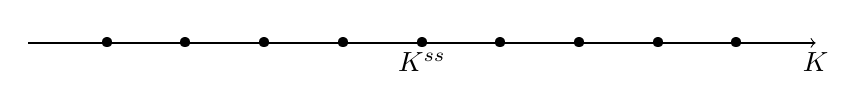
\begin{tikzpicture}
        \draw[->] (0, 0) -- (10, 0);
        \node[below] at (10, 0) {$K$};
        \foreach \Point in {(1, 0), (2, 0), (3, 0), (4, 0), (5, 0), (6, 0), (7, 0), (8, 0), (9, 0)}{
          \node at \Point {\textbullet};
        }
        \node[below] at (5, 0) {$K^{ss}$};
      \end{tikzpicture}
    \end{figure}

    \vfill\pause

    Takeaway: a grid samples points over an abstract set \hfill \textcolor{gray}{(desirably around an interesting point)}

    \vfill

    \hfill \gotobutton{apx:grid_example}{Example}

  \end{frame}

  \begin{frame}
    \frametitle{The VFI algorithm} \label{sld:vfi_algo}

    At iteration $j$, with a guess for $V^{(j)}(K)$

    \vfill\pause

    \begin{enumerate}
      \item For every \textit{potential} choice of $K'$
        \begin{enumerate}
          \item Compute the corresponding consumption $C$ using the budget constraint
          \item Enforce the non-negativity constraints (e.g., with a \texttt{NaN})
          \item Compute $u(C) + \beta V^{(j)}(K)$
        \end{enumerate}
      \vfill\pause
      \item Choose the value of $K'$ that maximizes the objective
        \begin{itemize}
          \item The ``max'' is $V^{(j+1)}(K)$
          \item The ``argmax'' is $K'\vphantom{K}^{(j+1)}(K)$
        \end{itemize}
      \vfill\pause
      \item Compute $\Delta \equiv \max \left( \left| V^{(j+1)}(K) - V^{(j)}(K) \right| \right)$
        \begin{itemize}
          \item If $\Delta \geq \varepsilon$, repeat 1--4 using $V^{(j+1)}(K)$ as a new guess
          \item If $\Delta < \varepsilon$, finish
        \end{itemize}
    \end{enumerate}

    \vfill

    \hfill\gotobutton{apx:numerical_objects}{Into the Numerical Objects}

  \end{frame}

  \begin{frame}
    \frametitle{Remarks}

    \textbf{Pros}
    \begin{itemize}
      \item Surely converges, always
      \item Relatively easy to code
      \item Returns the value function (useful for welfare analyses)
      \item Works for finite-horizon problems, discrete choice models, etc.
    \end{itemize}

    \vfill\pause

    \textbf{Cons}
    \begin{itemize}
      \item Suffers from the \textit{Curse of Dimensionality}
      \item Possibly the slowest method of all
    \end{itemize}

    \vfill\pause

    \textbf{Observations}
    \begin{itemize}
      \item The maximization step takes time
      \item Can parallelize: algorithm for finding $K'(k_i)$ is independent of $K'(k_j)$
    \end{itemize}
  \end{frame}

  \begin{frame}
    \frametitle{Policy Function Iteration (a.k.a., Howard Improvement)}

    \textbf{Observation:} at the ``true'' policy functions $C(K)$ and $K'(K)$, $V(\cdot)$ satisfies
    \begin{equation*}
      V(K) = u(C(K)) + \beta V(K'(K))
    \end{equation*}

    \vfill\pause

    Looking in terms of vectors and matrices
    \begin{align*}
      \mathbf{V} &= u(\mathbf{C}) + \beta \mathbf{Q} \mathbf{V} \\
      \mathbf{V} &= {\left[ \mathbf{I} - \beta \mathbf{Q} \right]}^{-1} u(\mathbf{C}) = \sum_{t=0}^{\infty} \beta^t u(C_t^*)
    \end{align*}

    \vfill\pause

    What is $\mathbf{Q}$? A sparse matrix regulating transitions from $K$ to $K'$\dots\ related to $K'(K)$
    \begin{equation*}
      Q_{i,j} = 1 \left( K = k_i \wedge K' = k_j \right)
    \end{equation*}

  \end{frame}

  \begin{frame}
    \frametitle{The PFI algorithm}

    At iteration $j$, with a guess for $K'^{(j)}(K)$

    \vfill\pause

    \begin{enumerate}
      \item Back out the the implied value function $\mathbf{V}$
        \begin{enumerate}
          \item Derive the matrix $\mathbf{Q}$ from the guess $K'^{(j)}(K)$
          \item Compute consumption $C$ from the budget constraint
          \item Enforce non-negativity constraints
          \item Compute $\mathbf{V} = {\left[ \mathbf{I} - \beta \mathbf{Q} \right]}^{-1} u(\mathbf{C})$
        \end{enumerate}
      \vfill\pause
      \item For every \emph{potential} choice of $K'$
        \begin{enumerate}
          \item Compute consumption $C$ from the budget constraints
          \item Enforce non-negativity constraints
          \item Compute $u(C) + \beta \mathbf{V}$
        \end{enumerate}
      \vfill\pause
      \item Choose the value $K'$ that maximizes the objective
        \begin{itemize}
          \item The ``argmax'' is $K'^{(j+1)}(K)$
        \end{itemize}
      \vfill\pause
      \item Compute $\Delta \equiv \max \left(  \left| K'^{(j+1)}(K) - K'^{(j)}(K) \right| \right)$
        \begin{itemize}
          \item If $\Delta \geq \varepsilon$, repeat 2--5 using $K'^{(j+1)}(K)$ as a new guess
          \item If $\Delta < \varepsilon$, finish
        \end{itemize}
    \end{enumerate}

  \end{frame}

  \begin{frame}
    \frametitle{Remarks about PFI}

    \textbf{Pros}
    \begin{itemize}
      \item Convergence has been proven, always
      \item Returns the value function (useful for welfare analyses)
      \item Is faster than VFI if the contraction modulus of $\mathbf{T}$ is close to unity
    \end{itemize}

    \vfill\pause

    \textbf{Cons}
    \begin{itemize}
      \item Suffers from the \textit{Curse of Dimensionality}
      \item May be slower than VFI, difficult to check ex-ante
      \item The initial condition may matter
      \item Infeasible for time-varying policy functions, discrete choice models, finite-horizon problems
    \end{itemize}

    \vfill\pause

    \textbf{Observations}
    \begin{itemize}
      \item The maximization step takes time
      \item Inverting $[ \mathbf{I} - \beta \mathbf{Q} ]$ may be computationally expensive
      \item Can parallelize the maximization step for each $K$
    \end{itemize}

  \end{frame}

  \begin{frame}
    \frametitle{Direct Projection}

    Compute the first-order conditions of the maximization problem
    \begin{equation*}
      \begin{cases}
        C(K) = C(K'(K)) {\left( \beta \alpha K'(K)^{\alpha-1} + 1 - \delta \right)}^{-\frac{1}{\gamma}} \\
        C(K) + K'(K) = K^{\alpha} + (1 - \delta) K
      \end{cases}
    \end{equation*}

    \vfill\pause

    \begin{itemize}
      \item Solve for $C(K)$: Can ask the computer the find the zero of the (functional) Euler equation
      \item Solve for $K'(K)$: Use the second equation
    \end{itemize}

    \vfill\pause

    \textbf{Catch:} These are \textit{functional} equations
    \begin{itemize}
      \item Choosing $C(K)$\dots \hfill \textcolor{gray}{meaning, choosing $\mathbf{C}$}
      \item \dots\ implies choosing $K'(K)$ from the budget constraint\dots \hfill \textcolor{gray}{meaning, obtaining $\mathbf{K'}$}
      \item \dots\ which implies something for $C(K'(K))$ \hfill \textcolor{gray}{\dots no way of doing this numerically!}
    \end{itemize}

    \vfill\pause

    \textbf{Workaround:} Given an initial condition, interpolate $C(K)$ and recompute points on $C(K'(K))$

  \end{frame}

  \begin{frame}
    \frametitle{Remarks about Direct Projection}

    \textbf{Pros}
    \begin{itemize}
      \item Zero-finding routine easily available in \texttt{scipy}
      \item May be faster than VFI/PFI
    \end{itemize}

    \vfill\pause

    \textbf{Cons}
    \begin{itemize}
      \item Convergence \textbf{not} guaranteed
      \item May be numerically inaccurate
    \end{itemize}

    \vfill\pause

    \textbf{Observations}
    \begin{itemize}
      \item Cannot be parallelized (if it uses interpolation over the grid)
      \item Checking accuracy requires solving with alternative methods\dots
    \end{itemize}

  \end{frame}

  \begin{frame}
    \frametitle{Practice time}

    Moving to a Jupyter Notebook

  \end{frame}

  \begin{frame}
    \frametitle{Exercises}

    \begin{enumerate}
      \item Use the code I showed you for VFI, keeping all the calibration values and parameters
        \begin{enumerate}
          \item Plot the no.~of iterations required for convergence against the no.~of points on the grid (e.g., $N \in \{50, 100, 150, \ldots, 1000\}$)
          \item Plot the no.~of iterations required for convergence against the value of $\beta$ (e.g., $\beta \in [0.75, 1)$)
          \item What can you say about speed of convergence of the VFI algorithm?
        \end{enumerate}
      \vfill
      \item Write your own code to implement Howard's Improvement (PFI) as in the slide above (i.e., do not use the shortcut I showed in the practice code in class)
        \begin{enumerate}
          \item Plot the no.~of iterations required for convergence against the value of $\beta$ (e.g., $\beta \in [0.75, 1)$)
          \item What can you say about the speed of PFI relative to the speed of VFI?
        \end{enumerate}
      \vfill
      \item Use the code I showed you for the Direct Projection method. Change the initial condition for the policy function with arbitrary choices. What can you say about the sensitivity of the algorithm w.r.t.~the initial condition?
      \vfill
      \item In what sense does any of the methods of this class deliver an approximation of the ``true'' value function?
    \end{enumerate}

  \end{frame}


  \appendix

  \begin{frame}
    \frametitle{Vectors, Domains and Functions in Computers} \label{apx:grid_example}

    Consider $f : X \to Y$, with $X, Y \subseteq \mathbb{R}$, such that $y = \sqrt{x}$ (i.e., $f(\cdot) \equiv \sqrt{\cdot}$)

    \vfill

    \begin{align*}
      X &\equiv
      \begin{bmatrix}
        x_1 & x_2 & \cdots & x_n
      \end{bmatrix}'
      &
      Y &\equiv
      \begin{bmatrix}
        y_1 & y_2 & \cdots & y_n
      \end{bmatrix}'
      &
      \text{with } y_i = \sqrt{x_i},\ \forall\ i \in \{1, 2, \ldots, n\}
    \end{align*}

    \vfill

    \begin{columns}
      \begin{column}{0.475\textwidth}
        \texttt{import numpy as np} \\
        \texttt{import matplotlib.pyplot as plt} \\
        \texttt{X = np.linspace(0, 1.2, num=5)} \\
        \texttt{Y = np.sqrt(X)} \\
        \texttt{plt.plot(X, Y)}
      \end{column}
      \begin{column}{0.375\textwidth}
        \begin{figure}
          \centering
          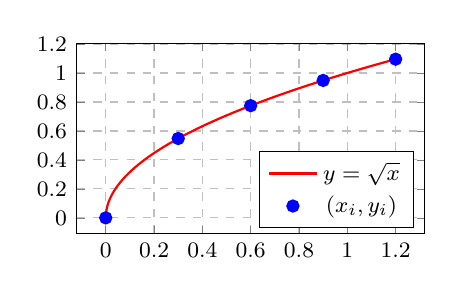
\begin{tikzpicture}
            \begin{axis}[footnotesize, width=6cm, height=4cm, legend pos=south east, domain=0:1.2, xmajorgrids=true, ymajorgrids=true, grid style=dashed]
              \addplot[samples=300, mark=none, red, thick]{sqrt(x)};
              \addlegendentry{$y=\sqrt{x}$};
              \addplot[samples=5, only marks, blue, thick]{sqrt(x)};
              \addlegendentry{$(x_i, y_i)$};
            \end{axis}
          \end{tikzpicture}
        \end{figure}
      \end{column}
    \end{columns}

    \vfill

    \hfill \backbutton{sld:grid}

  \end{frame}

  \begin{frame}
    \frametitle{Peeking into Numerical Objects with VFI}
    \label{apx:numerical_objects}

    Convention: rows are states, columns are controls

    \vfill

    The budget constraint
    \begin{align*}
      \underbrace{\begin{bmatrix}
        k_1^\alpha \\ k_2^\alpha \\ \vdots \\ k_n^\alpha
      \end{bmatrix}}_{K^\alpha}
      + (1 - \delta)
      \underbrace{\begin{bmatrix}
        k_1^\alpha \\ k_2^\alpha \\ \vdots \\ k_n^\alpha
      \end{bmatrix}}_{K}
      -
      \underbrace{\begin{bmatrix}
        k_1 & k_2 & \cdots & k_n
      \end{bmatrix}}_{K'}
      &=
      \underbrace{\begin{bmatrix}
        c_{1,1} & c_{1,2} & \cdots & c_{1,n} \\
        c_{2,1} & c_{2,2} & \cdots & c_{2,n} \\
        \vdots  & \vdots  & \ddots & \vdots  \\
        c_{n,1} & c_{n,2} & \cdots & c_{n,n} \\
      \end{bmatrix}}_{C}
    \end{align*}

    \vfill

    The value function (to be maximized---keep best element in each row)
    \begin{align*}
      \underbrace{\begin{bmatrix}
        \tilde{V}_{1,1} & \tilde{V}_{1,2} & \cdots & \tilde{V}_{1,n} \\
        \tilde{V}_{2,1} & \tilde{V}_{2,2} & \cdots & \tilde{V}_{2,n} \\
        \vdots   & \vdots   & \ddots & \vdots   \\
        \tilde{V}_{n,1} & \tilde{V}_{n,2} & \cdots & \tilde{V}_{n,n} \\
      \end{bmatrix}}_{\tilde{V}(K, K')}
      &=
      \underbrace{\begin{bmatrix}
        u(c_{1,1}) & u(c_{1,2}) & \cdots & u(c_{1,n}) \\
        u(c_{2,1}) & u(c_{2,2}) & \cdots & u(c_{2,n}) \\
        \vdots  & \vdots  & \ddots & \vdots  \\
        u(c_{n,1}) & u(c_{n,2}) & \cdots & u(c_{n,n}) \\
      \end{bmatrix}}_{u(C)}
      + \beta
      \underbrace{\begin{bmatrix}
        V(k_1) & V(k_2) & \cdots & V(k_n)
      \end{bmatrix}}_{V(K')}
    \end{align*}

    \vfill

    \vfill

    \textcolor{gray}{(Linear algebra doubts? Broadcasting!)}
    \hfill
    \backbutton{sld:vfi_algo}

  \end{frame}



\end{document}
